%%%%%%%%%%%%%%%%%%%%%%%%%%%%%%%%%%%%%%%%%%%%%%%%%%%%%%%%%%%%%%%%%%%%%%%%%%%%%%%%%
%
% Purpose:  Introduction for the Planetary model.
%
% 
%
%%%%%%%%%%%%%%%%%%%%%%%%%%%%%%%%%%%%%%%%%%%%%%%%%%%%%%%%%%%%%%%%%%%%%%%%%%%%%%%%


%\section{Purpose and Objectives of \PlanetaryDesc}
% Incorporate the intro paragraph that used to begin this Chapter here. 
% This is location of the true introduction where you explain what this model 
% does.
\label{ch:planetaryintro}
The \PlanetaryDesc\ provides the state of a vehicle in three different representations:
\begin{itemize}
\item{Cartesian coordinates}\ \newline
 Cartesian coordinates are centered and fixed with the planet
\item{Spherical coordinates}\ \newline
These are centered on the planet, with $\phi$ measured from the Cartesian z-axis, and $\theta$ measured in the Cartesian x-y plane from the Cartesian x-axis toward the Cartesian y-axis.  The position is represented as \textit{latitude} ($\frac{\pi}{2} - \phi$), \textit{longitude} ($\theta$), and \textit{altitude} ($r - r_{equatorial}$).
\item{Elliptical coordinates}\ \newline
These are also centered on the planet, with elliptical longitude and latitude being measured to the point on the reference ellipsoid (surface) that has a normal that passes through the point of interest.  See Figure~\ref{fig:planetaryellipticalspherical} for a graphical distinction between spherical and elliptical coordinates.
\end{itemize}

\begin{figure}[htp]
\begin{center}
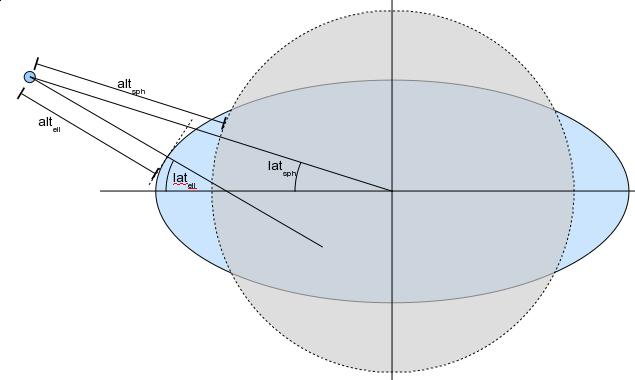
\includegraphics[width=5in]{figures/sphericalelliptical.jpg}
\caption{The differences between spherical and elliptical altitude and latitude.}
\label{fig:planetaryellipticalspherical}
\end{center}
\end{figure}












